
\documentclass[12pt]{report}
\usepackage[utf8]{inputenc}

\usepackage{geometry}
\usepackage[spanish]{babel}
\renewcommand{\baselinestretch}{1.5}
\geometry{letterpaper, margin=2.5cm}
\usepackage{graphicx}
\usepackage{hyperref}
\urlstyle{same}
\usepackage{fancyhdr}
\usepackage{amsmath}
\usepackage{braket,mleftright}
\mleftright
 
\usepackage[sorting=none]{biblatex}
 
\addbibresource{references.bib}

\begin{document}

\begin{titlepage}
   \begin{center}
       \vspace*{1cm}
       
       
       \large
       \textbf{Estimación del ruido generado por el \textit{forward scattering} de rayos cósmicos secundarios en un detector Cherenkov de agua}
       
       %\large
       %\vspace{0.5cm}
        %¿Subtítulo?
 
       \vspace{1.5cm}
 
       \small
       Propuesta de tesis de pregrado para optar al título de \\
       Físico
       
       
       \normalsize
       \textbf{Ricardo de León Barrios}
       
       \small
       \vspace{1cm}
       Director\\
       \textbf{Mauricio Suárez Durán}$^1$\\
       Doctor en Ciencias Naturales (Física)
       
       \vspace{1cm}
       Codirector\\
       \textbf{Luis A. Núñez de Villavicencio}$^1$\\
       Doctor en Física\\
       
       \vspace{1cm}
       $^1$\textit{Grupo de Investigación en Relatividad y Gravitación, UIS}
 
       \vfill
       
       
 
       %\vspace{0.8cm}
 
       
 
       \small
       Escuela de Física\\
       Facultad de Ciencias\\
       Universidad Industrial de Santander\\
       Bucaramanga, Colombia\\
       2020\\
       \vspace{0.3cm}
       
\includegraphics[width=0.25\textwidth]{logo/logoUIS.png}
 
   \end{center}
\end{titlepage}

%---------------------------------------

\section*{Resumen}


%------------------------------------
%\section*{¿Introducción?}


%-------------------------------------------
\section*{Planteamiento del problema y justificación}

La muografía ha despertado el interés de la comunidad científica en los últimos años debido a su gran poder en aplicaciones de escaneo de grandes estructuras.

El principio en el que se basa la muografía es sencillo: similar a como los rayos x en medicina se atenúan en distintos valores cuando pasan por las diferentes estructuras internas del cuerpo, el flujo de muones sobre un detector también varía en función de la cantidad de materia que los muones han atravesado en su trayectoria. El uso de muones presenta una importante ventaja para el escaneo de estructuras geológicas debido al gran poder penetrativo de estas partículas así como al hecho de que están fácilmente disponibles en grandes cantidades: los muones están siendo creados constantemente en la atmósfera terrestre debido a la interacción de rayos cósmicos con partículas de aire, en procesos llamados \textit{cascadas atmosféricas extensas}.

Con la muografía aplicada al escaneo de estructuras geológicas se pretende obtener modelos de la distribución de densidades en los objetos escaneados a partir de la variación en el flujo de muones que atraviesan las estructuras y son recibidos en un detector.

Con detectores Cherenkov se puede detectar el paso de partículas energéticas, como los muones, basándose en el fenómeno de emisión de radiación Cherenkov, mientras que con hodoscopios se puede hacer una recreación de la trayectoria de las partículas incidentes. Con esto en mente, la Universidad Industrial de Santander y colaboradores han estado trabajando en el proyecto MuTe\footnote{\textit{\textbf{Mu}on \textbf{Te}lescope}}: la implementación de un detector de muones híbrido que combine los principios de funcionamiento de un hodoscopio con un detector Cherenkov de agua (WCD\footnote{\textit{Water Cherenkov Detector}}) para el escaneo de estructuras geológicas en las montañas de Colombia \cite{rodriguez2018minimute}. En representación de Colombia, la UIS realiza el estudio del clima espacial y la coordinación de proyectos de implementación de detectores como el MuTe para mediciones de radiación cósmica a nivel del suelo dentro del marco del proyecto LAGO\footnote{\textit{Latin American Giant Observatory}, \url{http://lagoproject.net/}}. Supervisado por la Colaboración LAGO, una colaboración entre más de 100 científicos en 30 instituciones de 11 países distintos (en su mayoría latinoamericanos)\footnote{Los países que participan en la Colaboración LAGO son Argentina, Bolivia, Brasil, Chile, Colombia, Ecuador, Guatemala, México, Perú y Venezuela en Latinoamérica, y España en Europa.}, el proyecto LAGO pretende servir como un gran observatorio de astropartículas, haciendo investigación en temas de Universo extremo, clima espacial y radiación atmosférica a nivel del suelo.

En particular, uno de los objetivos del proyecto MuTe es estudiar la estructura de los volcanes activos en Colombia. Estudiando las distribuciones de densidad en los volcanes activos del país, se espera obtener modelos de sus estructuras internas que, potencialmente, permitan evaluar los riesgos futuros que estos puedan representar. Para esto, se busca que las imágenes obtenidas de los volcanes por tomografía de muones sean lo más detalladas posibles, siendo entonces importante reducir tanto como sea posible los efectos del ruido en los detectores.

Cuando se hace muografía de estructuras geológicas, existen varias fuentes de ruido que afectan la imagen: hadrones cargados y electrones y positrones, conocidos como \textit{muones falsos} (\textit{fake muons}), y los llamados \textit{muones suaves} (\textit{soft muons}) que se ``reflejan'' en la superficie escaneada y llegan al detector, como se muestra en la figura \ref{fig:scatteredNoise}. También pueden llegar muones por detrás del detector (\textit{backward muons}), quienes igualmente sumarán al ruido de fondo \cite{bonechi2020atmospheric}.

\begin{figure}
    \centering
    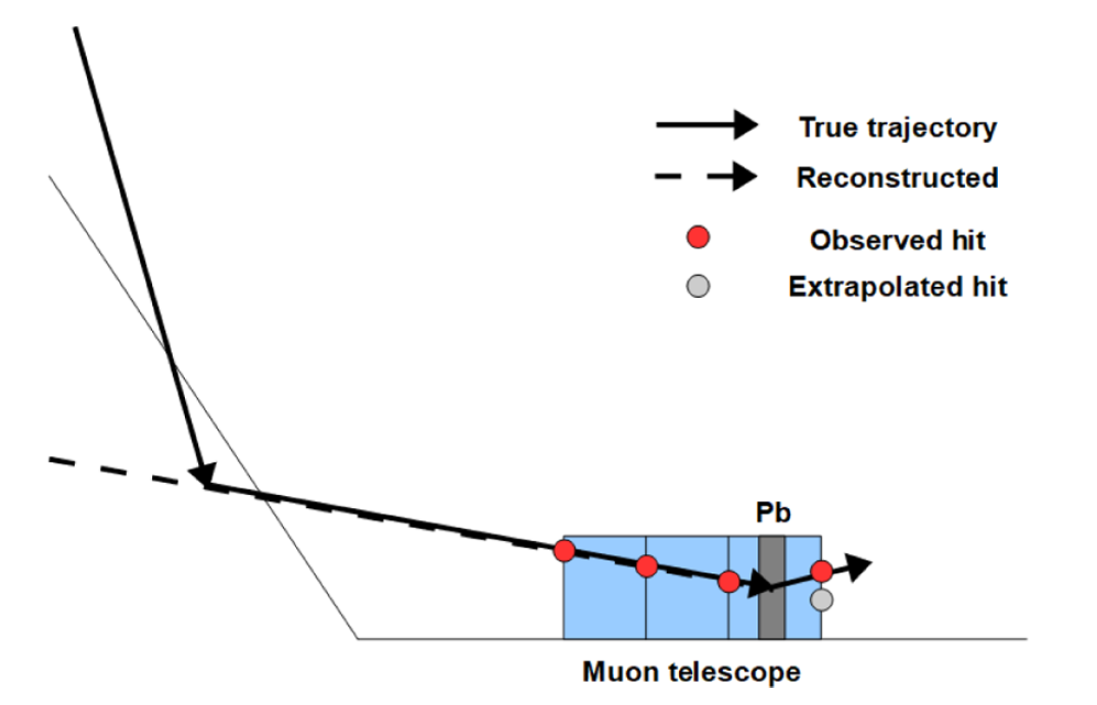
\includegraphics[width=3.5in]{images/scatteredNoiseV2.png}
    \caption{Muon dispersado por la superficie del volcán genera ruido en el WCD. Imagen tomada de (L Bonech y col. 2020) \cite{bonechi2020atmospheric}.}
    \label{fig:scatteredNoise}
\end{figure}

El MuTe puede discrimar electrones/positrones de muones mediante técnicas de identificación de partículas. Por ejemplo, como se ve en simulaciones hechas en (H Asorey y col. 2017) \cite{asorey2017muon}, la gran mayoría de positrones y electrones se encuentran en un rango energético inferior a los muones. Aplicando un umbral a la energía de las partículas recolectadas por el detector se puede reducir en gran medida el efecto de los electrones y positrones en la imagen.

Reducir el efecto del ruido generado por los muones dispersados por \textit{forward scattering} es un poco más complejo. En general, el efecto de los muones dispersados es insignificante a altas energías pero cobra importancia a bajas energías. Estos muones dispersados de bajas energías llegan al detector donde se reconstruye su trayectoria, la cual apunta de vuelta a la estructura estudiada, haciendo que se mimeticen con aquellos muones que sí atravesaron el objeto, alterando nuestra percepción de su densidad en esa dirección. Debido a que estas partículas son también muones, no pueden ser descartados del conteo detectado mediante técnicas de identificación de partículas, representando potencialmente un ruido irreducible \cite{gomez2017forward}.

Teniendo en cuenta lo anterior, este trabajo de grado se enfocará en caracterizar el ruido creado por el \textit{forward scattering} de muones en un WCD. Mediante herramientas computacionales, se simularán los efectos que estas partículas dispersadas tienen sobre los detectores, cómo afectan a la obtención del perfil de densidad de las estructuras escaneadas y cómo se podría reducir su impacto en la imagen. Con esto, se busca ayudar a que los mapas de densidad de estructuras geológicas, como volcanes, medidos por muografía, sean lo más prolijos posible, facilitando su estudio y permitiendo, potencialmente, una valoración detallada de los posibles riesgos que estos puedan suponer para la población.



%--------------------------
\section*{Marco teórico}

\subsection*{Sobre rayos cósmicos y cascadas atmosféricas extensas}

\normalsize

Los rayos cósmicos son partículas cargadas y altamente energéticas provenientes del espacio. Se pueden clasificar entre aquellas provenientes de nuestro propio Sol y de fuentes externas al sistema solar, ya sea dentro de la Vía Láctea, o de fuentes extragalácticas \cite{moldwin2008introduction}. A pesar de que se les denomina \textit{rayos}, comúnmente se excluye de esta definición a la radiación electromagnética \cite{NASACosmicopia}, limitándose exclusivamente a partículas con masa. La mayoría de los rayos cósmicos están compuestos por núcleos de elementos que van desde el más ligero, el hidrógeno, hasta núcleos de elementos pesados, como el hierro. También se incluyen otras partículas como electrones, neutrones, neutrinos, positrones y antiprotones \cite{NASAImagine}.

Las partículas de rayos cósmicos pueden llegar a alcanzar energías muy altas, de alrededor de 100 MeV, y velocidades de más del 99\% de la velocidad de la luz \cite{moldwin2008introduction}. Estas partículas formadas en eventos astrofísicos como llamaradas solares y supernovas se denominan \textbf{partículas primarias}. Cuando llegan a la atmósfera terrestre, interactúan con moléculas de aire (principalmente nitrógeno, oxígeno y argón, que son los mayores componentes de la atmósfera) y decaen en \textbf{partículas secundarias}, creando eventos llamados \textit{cascadas atmosféricas extensas}, o \textit{EAS}\footnote{\textit{Extensive Air Showers}.}. Estas partículas secundarias tienen menos energía que las primarias que las crearon. Algunas partículas secundarias que se pueden formar en estas cascadas son piones y kaones, que a su vez, pueden decaer en muones y neutrinos \cite{grieder2010extensive}. También se pueden formar cascadas electromagnéticas (fotones), partículas alfa, protones, electrones y neutrones.

Para el estudio de los rayos cósmicos es importante la noción de flujo, que se define como el número de partículas que atraviesan una superficie por unidad de área, por unidad de tiempo. En el caso del flujo de rayos cósmicos en la parte superior de la atmósfera, existen varios factores que lo pueden afectar, tales como la actividad solar y el campo magnético terrestre \cite{PhysRevD.98.030001}.

De particular interés en la actualidad es el estudio del flujo de muones, con importantes aplicaciones para escaneos por radiografía y tomografía, de los cuales se hablará más a fondo en la siguiente sección. Los muones generalmente se forman por el decaimiento de piones, quienes a su vez se crean a partir del choque de núcleos atómicos de rayos cósmicos con partículas de la atmósfera. Los muones son bastante inestables, decayendo rápidamente por interacción débil. El tiempo de vida de los muones, medido en un marco de referencia inicial en reposo respecto a ellos, solo permitiría una distancia de viaje de menos de 500 metros para la mitad de estos (viajando al 99,97\% de la velocidad de la luz) antes de decaer en otras partículas; esto es sin tener en cuenta los efectos relativistas. Sin embargo, debido a las altas velocidades que alcanzan los muones, se deben tener en cuenta los efectos de la contracción de longitudes y la dilatación del tiempo. En este caso, desde nuestra perspectiva en la Tierra, la semivida de los muones se extiende debido a la dilatación temporal, siendo lo suficientemente larga como para detectarlos en la superficie de la Tierra, e incluso a varios cientos de metros bajo tierra, debido a su alto poder penetrativo. Desde la perspectiva de un marco de referencia inercial en reposo respecto de los muones, actúa la contracción espacial, haciendo que la distancia de viaje hacia la superficie de la Tierra sea más corta \cite{cunningham2019high}.

Dos principales métodos de detección de rayos cósmicos existen: uno de detección directa de las partículas primarias en la parte superior de la atmósfera, mediante el uso de globos de grandes altitudes y satélites, y un segundo método, que consiste en detectar, a nivel del suelo, las partículas secundarias y la radiación electromagnética creadas en las EAS. Estas formas de detección son denominadas detección \textit{directa} e \textit{indirecta}, respectivamente. El presente trabajo de investigación se asienta sobre el método de detección indirecta a nivel del suelo.

Una de las herramientas más importantes en la detección de partículas secundarias es el detector Cherenkov, cuyo funcionamiento se basa en el fenómeno de la radiación de Cherenkov: Así llamada por el físico soviético Pável Cherenkov, es la radiación electromagnética emitida cuando un medio dieléctrico es atravesado por una partícula cargada viajando a una velocidad superior a la de la luz en ese medio \cite{jelley1955cerenkov}. Este fenómeno se puede entender como un análogo electromagnético a la onda de choque que se crea cuando un objeto viaja a una velocidad que supera a la velocidad del sonido en un medio.

%---------------------------------------------------------


\subsection*{Sobre la muografía}

La muografía (lit. 'escribir con muones') es el uso de muones cósmicos de altas energías para aplicaciones de escaneo. La muografía ha despertado el interés de la comunidad científica, realizándose importantes avances en esta tecnología en las últimas dos décadas y desarrollando aplicaciones tanto comerciales como académicas \cite{kaiser2019muography}. El uso de muones para escaneo presenta importantes ventajas; entre ellas, el hecho de que estas partículas son muy abundantes en la Tierra, produciéndose en EAS en la atmósfera.

El principio en el que se basa la muografía es similar al uso de rayos X en la medicina como indicador de la densidad de las estrucutras óseas del cuerpo. En el caso de la muografía, se usan muones, provenientes de rayos cósmicos, como indicadores de la densidad de estructuras, generalmente de gran tamaño. Debido a esto, es muy frecuente el uso del término \textit{radiografía de muones}, especialmente para referirse al escaneo en dos dimensiones; por otro lado, para la creación de imágenes tridimensionales se prefiere el término \textit{tomografía de muones} \cite{kaiser2019muography}.

La forma en la que se crean mapas de estructuras por medio de muografía es estudiando la atenuación del flujo de muones que pasan a través de ellas. El objeto que se desee estudiar presentará una opacidad ante el paso de muones, que depende de su densidad. Esta opacidad se puede deducir a partir de la atenuación, la cual se halla comparando el flujo de muones a través de la estructura con el flujo de muones en condiciones de cielo abierto. Los muones pierden energía por interacciones débiles con la materia a través de la cual pasan, principalmente por medio de ionización. Esta pérdida de energía para un cierto material está relacionada con la energía mínima que deben tener los muones para cruzar la estructura, y esta a su vez está relacionada con el flujo integrado de muones. A lo largo de su recorrido a través de la materia, los muones también pueden verse dispersados por medio de dispersión de Coulomb. \cite{lesparre2010geophysical}.

La muografía representa entonces una herramienta útil para realizar mapas de densidad de estructuras que se deseen estudiar. Sus aplicaciones se encuentran generalmente en la geociencia, seguridad nuclear, ingeniería civil y arqueología. La figura \ref{fig:applications} muestra una infografía esquemática con distintas aplicaciones de la muografía. En la geociencia en particular, una de sus más importantes aplicaciones es en el escaneo de volcanes para comprender mejor sus estructuras y evaluar sus posibles riesgos.

Los volcanes son puntos en la superficie de la Tierra por donde se puede presentar la salida de material magmático proveniente del interior de esta. La formación y erupción de un volcán responde a un largo proceso geológico de miles a millones de años \cite{vesga2018inversion}. En los últimos años, la muografía ha surgido como una herramienta de estudio de estas estructuras; de su génesis, su funcionamiento y su evolución.

\begin{figure}
    \centering
    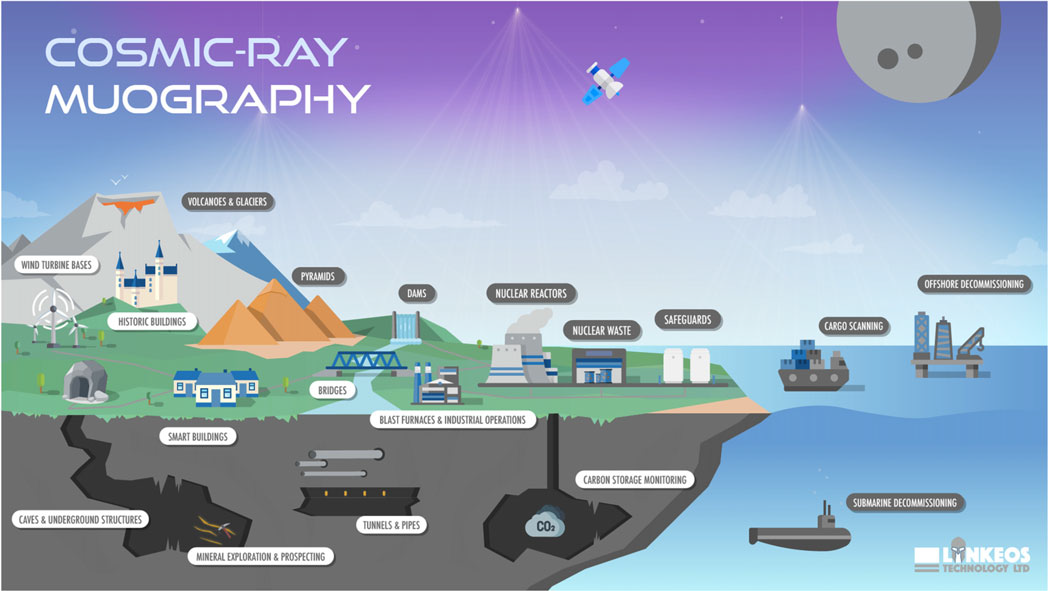
\includegraphics[width=0.9\textwidth]{images/applications.png}
    \caption{Aplicaciones de la muografía. Imagen tomada de (R Kaiser, 2019) \cite{kaiser2019muography}.}
    \label{fig:applications}
\end{figure}

La vulcanología está estrechamente emparentada con el estudio de la corteza terrestre. La corteza es una delgada capa rocosa que cubre la superficie de la Tierra, siendo la capa más externa de la \textbf{geósfera} o tierra sólida. Se separa en dos tipos principales: oceánica y continental. La oceánica tiene un grosor promedio de 6 km, densidad promedio de 3 g cm$^{-3}$ y una edad de menos de 200 millones de años, mientras que la continental tiene un grosor promedio de 39 km, densidad promedio de 2,84 g cm$^{-3}$ y edad promedio de 1500 millones de años \cite{mooney20101}. La corteza terrestre \textit{flota} sobre el manto, teniendo este una densidad mayor. Puesto que la corteza oceánica tiene mayor densidad que la corteza continental, esta última \textit{flota más alto}, y los cuerpos masivos de agua se acumulan sobre la corteza oceánica. Esta condición de equilibrio entre corteza y manto se denomina isostasia. Los elementos más abundantes en la corteza son el oxígeno, el silicio y el aluminio, y los minerales más abundantes son los feldespatos, el cuarzo y los piroxenos \cite{anderson2010geomorphology}.

En este trabajo estudiaremos la interacción de las partículas de las EAS con la materia de la corteza terrestre, la cual modelaremos como la denominada \textit{roca estándar}. Esta es una representación genérica del suelo bastante usada en la física de partículas y rayos cósmicos, y el estudio de escaneo de terrenos mediante muones, en la que se define que la roca está constituida por un material de densidad 2,65 g cm$^{-3}$ aproximadamente, y que cumple las relaciones $\langle Z/A \rangle=0.5$ y $\langle Z^2/A \rangle=5.5$, donde $Z$ y $A$ son el número atómico y el número másico del elemento constituyente, respectivamente \cite{groom2001muon}.

En particular, estamos interesados en el fenómeno de \textit{forward scattering} de muones que produce ruido en los detectores. Los muones que son dispersados por \textit{forward scattering} y llegan al detector entorpecen el proceso de escaneo de estructuras geológicas ya que generan señales falsas que no provienen de muones que atravesaron la estructura, como se muestra en la figura \ref{fig:scatteredNoise}. Es entonces importante caracterizar este ruido en un detector de muones con el fin de reducir su efecto sobre las imágenes de densidades que se deseen tomar de estructuras geológicas. Para esto, se hará uso de múltiples herramientas computacionales para simular y analizar estos efectos. Las herramientas que se utilizarán en el proyecto para las simulaciones son CORSIKA, MAGNETOCOSMICS y Geant4.


%---------------------------------------

\subsection*{Sobre CORSIKA, MAGNETOCOSMICS y Geant4}

CORSIKA\footnote{\textit{\textbf{CO}smic \textbf{R}ay \textbf{SI}mulations for \textbf{KA}scade}} es un programa computacional utilizado para simular EAS causadas por rayos cósmicos energéticos. El software utiliza métodos de Montecarlo para simular las interacciones de partículas de rayos cósmicos con la atmósfera terrestre. Las partículas son rastreadas a lo largo de la atmósfera mientras son sujetas a interacciones con los núcleos de aire y procesos de decaimiento.

El programa hace uso de múltiples modelos diferentes para simular las interacciones, tales como VENUS, QGSJET, DPMJET y SIBYLL para interacciones hadrónicas a altas energías, GHEISHA, FLUKA y UrQMD para interacciones hadrónicas a bajas energías y una adaptación de EGS4 para interacciones electromagnéticas \cite{heck1998corsika}.

Este programa es de uso extendido en el estudio de rayos cósmicos, ya que permite una descripción detallada de las cascadas atmosféricas creadas por estos. La figura \ref{fig:ironcascade} muestra un ejemplo de una cascada producida por la interacción de un núcleo de hierro con la atmósfera, simulada en CORSIKA.

\begin{figure}
    \centering
    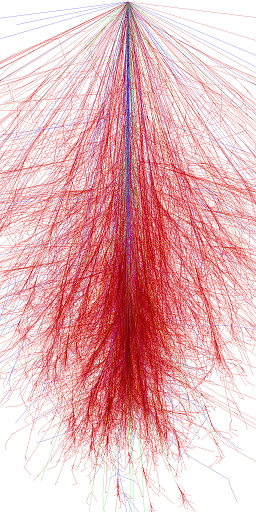
\includegraphics[width=1.5in]{images/ironcascade.png}
    \caption{Cascada atmosférica creada a partir de núcleo de hierro con energía de 1 TeV simulada en CORSIKA. Imagen tomada de \url{https://www.ikp.kit.edu/corsika/index.php}}
    \label{fig:ironcascade}
\end{figure}

Para la simulación de EAS, un aspecto importante es el modelo de rigidez atmosférica. El programa hace seguimiento, entre otras cosas, a la energía de las partículas de las EAS; si una partícula no tiene una energía lo suficientemente alta como para pasar el umbral establecido por el modelo de rigidez atmosférica, la partícula no podrá continuar su viaje a través de la atmósfera. Además, es bien sabido que el campo magnético terrestre puede afectar el viaje de los rayos cósmicos, alterando su curso y desviándolos de sus trayectorias iniciales. Estos son fenómenos cuyos efectos se pueden tener en cuenta en la simulación de EAS mediante la herramienta MAGNETOCOSMICS de Geant4.

La aplicación de MAGNETOCOSMICS permite calcular la trayectoria de partículas cargadas en la magnetosfera terrestre mediante modelos avanzados del campo geomagnético, y computar los modelos de rigidez atmosférica para el filtrado de partículas \cite{magnetocosmics}. La gran utilidad de esta herramienta hace menester integrarla con las simulaciones de CORSIKA.

Finalmente, Geant4\footnote{\textit{\textbf{GE}ometry \textbf{AN}d \textbf{T}racking}} es un grupo de herramientas computacionales (\textit{toolkit}) diseñadas para la simulación del paso de partículas a través de materia, simulando procesos de interacciones y decaimientos. Ha sido ampliamente utilizado en las áreas de física de partículas, física nuclear, física de aceleradores, física espacial y estudios médicos \cite{agostinelli2003geant4}.

En este trabajo balancearemos el uso de todas estas herramientas computacionales para simular con rigor la interacción de EAS con la materia de la corteza terrestre.



%---------------------------
%\subsection*{Estado del arte}










%---------------------------
%\section*{Plan de trabajo}





\section*{Objetivos}

\subsection*{General}
\begin{itemize}
    \item Estimar el flujo y espectro energético del ruido producido por el \textit{forward scattering} de rayos cósmicos secundarios en un detector Cherenkov de agua.
\end{itemize}

\subsection*{Específicos}
\begin{enumerate}
    \item Estimar las partículas secundarias producidas en EAS que llegan a interactuar con el suelo, teniendo en cuenta el efecto de desviación de rayos cósmicos ejercido por el campo geomagnético. Esto se hará documentando una herramienta de Python que integre los softwares de CORSIKA y MAGNETOCOSMICS para automatizar y simplificar el proceso de simulación de EAS.
    \item Modelar un volumen de material de suelo genérico correspondiente a \textit{roca estándar}.
    \item Obtener un modelo del \textit{forward scattering} de las partículas secundarias del numeral 1 simulando sus interacciones con la superficie de roca estándar del numeral 2 mediante las herramientas de simulación de Geant4.
    \item Estimar el flujo y espectro energético del ruido generado por el \textit{forward scattering} de partículas secundarias modelado en el numeral 3 en un detector Cherenvok de agua.
\end{enumerate}

\section*{Metodología}

\begin{enumerate}
    \item Se leerá y aprenderá sobre la teoría física pertinente para el desarrollo del proyecto; principalmente la teoría concerniente a rayos cósmicos, cascadas atmosféricas extensas, \textit{forward scattering} y detección de rayos cósmicos.
    \item Se entenderá y analizará el funcionamiento de los \textit{softwares} necesarios, con el fin de tener un buen manejo de estos para llevar a cabo el proyecto. Los programas en cuestión son CORSIKA y MAGNETOCOSMICS para la simulación de EAS, y Geant4 para la simulación de interacciones de partículas de las EAS con la materia del suelo.
    \item Se documentará un código en Python que integre los softwares de CORSIKA y MAGNETOCOSMICS para automatizar y simplificar el proceso de simulación de EAS en cualquier posición geográfica y época del año, para su utilización por la Colaboración LAGO. Con esto, se estimarán los rayos cósmicos secundarios producidos en EAS que alcanzan el suelo en un sitio de observación arbitrario.
    \item Se aprenderá sobre el tipo de roca a utilizar, llamada roca estándar, y se elaborará un modelo de esta basado en su composición química y demás características relevantes, que pueda ser usado para la simulación con Geant4.
    \item Mediante las herramientas disponibles de Geant4, se simulará la interacción de las EAS estimadas en el numeral 3 con el modelo de suelo (roca estándar) creado en el numeral 4 para obtener una descripción detallada del \textit{forward scattering} de partículas secundarias.
    \item Con los resultados obtenidos en el numeral 5, se estimará el flujo y espectro energético del ruido generado por el \textit{forward scattering} de rayos cósmicos secundarios en un detector Cherenkov de agua.
    \item Se escribirá el libro de tesis con la teoría, desarrollo y resultados del proyecto pertinentes.
\end{enumerate}

\section*{Cronograma de actividades}

\section*{Presupuesto}




%----------------------------
\printbibliography

\end{document}
